\documentclass[conference]{IEEEtran}
\usepackage[T1]{fontenc}
\usepackage{cite}
\usepackage{amsmath,amssymb,amsthm}
\usepackage{graphicx,booktabs,array,multirow,tabularx}
\usepackage{algorithmic}
\usepackage{tikz,pgfplots,pgfplotstable}
\usetikzlibrary{arrows.meta,positioning,calc,patterns}
\pgfplotsset{compat=1.18}
\usepackage[hidelinks]{hyperref}
\usepackage{microtype}
\hypersetup{pdftitle={MobiShard: Lifecycle-Aware Resource Reservation for Mobile Smart-Contract Validation},pdfsubject={Research manuscript and local reproducibility artifact}}
\newtheorem{proposition}{Proposition}
\newcounter{algorithm}
\makeatletter\let\tableinput\@@input\makeatother
\newcommand{\va}{\mathbf a}
\newcommand{\vh}{\mathbf h}
\newcommand{\vH}{\mathbf H}
\newcommand{\vq}{\mathbf q}
\newcommand{\vQ}{\mathbf Q}
\newcolumntype{L}[1]{>{\raggedright\arraybackslash}p{#1}}
\title{MobiShard: Lifecycle-Aware Resource Reservation\\for Mobile Smart-Contract Validation}
% Supplied manuscript authors and affiliations; verify before distribution.
\author{
\IEEEauthorblockN{Vipin Deval\IEEEauthorrefmark{1}\IEEEauthorrefmark{2},
Vimal Dwivedi\IEEEauthorrefmark{3},
Alex Norta\IEEEauthorrefmark{4}\IEEEauthorrefmark{5},
Dirk Draheim\IEEEauthorrefmark{2}}
\IEEEauthorblockA{\IEEEauthorrefmark{1}Department of Computer Science and Engineering,\\
Krishna Institute of Engineering \& Technology (KIET), Ghaziabad, India}
\IEEEauthorblockA{\IEEEauthorrefmark{2}Information Systems Group, Tallinn University of Technology, Tallinn, Estonia}
\IEEEauthorblockA{\IEEEauthorrefmark{3}Intelligent System Research Center, Center for Legal Technology,\\
Ulster University, United Kingdom}
\IEEEauthorblockA{\IEEEauthorrefmark{4}Tallinn University (TLU), Tallinn, Estonia\quad
\IEEEauthorrefmark{5}University of Pretoria (UP), Pretoria, South Africa}
\IEEEauthorblockA{Corresponding author: Vipin Deval (vipin.deval@taltech.ee)}
}

\begin{document}
\maketitle
\begin{abstract}
Mobile smart-contract requests can pass admission checks yet remain unfinished
when concurrent requests draw on the same budget. Checking each validation
stage prevents negative balances, but does not protect the allowance needed
by later stages. We present MobiShard, which atomically reserves each request's
remaining logical battery and computation costs before shard dispatch. Stage
charges reduce the reservation, and terminal handling releases any unused
portion. The design separates request origination, the charged account, and
execution placement. A budget invariant establishes conditional resource
feasibility under fixed costs and atomic updates. Selected guards and evidence
dependencies come from a Coloured Petri Net specification and inform a separate
implementation. We compare stagewise checking, full-path prechecking,
reservation, and per-participant serialization in a trusted, single-host
prototype with six services. The evaluation covers 880 trials and 225,280
submissions. In computation-limited bursts, reservation completes 80 of 256
requests per trial, compared with a mean of 72.40 for stagewise checking,
a 10.5\% increase. Serialization also reaches 80, but permits only one active
request per participant. In mixed-resource trials, both complete 96 requests;
reservation reduces mean trial elapsed time from 377.2 to 220.6\,ms. No clear
timing advantage is established in the main computation-limited comparison.
Modeled connectivity loss, however, interrupts more admitted requests under
reservation than under serialization. Reservation thus protects completion
capacity while allowing concurrent validation, but its runtime benefit depends
on the workload. These results concern logical budgets and local commitment,
not measured mobile-energy savings or consensus finality.
\end{abstract}

\begin{IEEEkeywords}
mobile smart contracts, resource reservation, admission control, sharding,
Coloured Petri Nets, concurrent validation
\end{IEEEkeywords}

\section{Introduction}

Edge assistance lets a mobile participant submit smart-contract requests and
inspect validation evidence without running the entire blockchain on its
device. Mobile smart-contract (MSC) participation still requires a sequence
of resource-consuming operations, which may run on different hosts and at
different times. Saguaro uses a hierarchy to process mobile-originated
transactions~\cite{saguaro}; permissioned sharding and cross-shard protocols
also divide processing among services~\cite{sharper,byshard,rivet}. A balance
read at admission therefore describes only part of the account's position.
The account may have enough allowance for the next operation while owing
resources to requests already in progress. We study those outstanding
obligations using logical charges to a participant's account, rather than
measurements of its device's physical resource consumption.

Consider several service-payment requests submitted by a mobile participant
during a short connectivity window. Each can pass the resource check for its
next validation stage. If they all spend on early stages before any finishes,
the account may be left with too little allowance for the remaining work.
No stage has overdrawn the account, yet the requests can collectively complete
fewer paths than the initial budgets could support. An admission check for
the full path has the same weakness when it records no commitment: until
consumption occurs, later requests can be checked against the same balance.
This is the difference between \emph{observing available resources} and
\emph{reserving the resources required to complete an admitted request}.
Throughout the paper, completion capacity means the number of requests that
the initial wallet and resource budgets can support through the configured
validation path.

Where a request executes and how its allowance is committed are separate
decisions. TxAllo optimizes transaction allocation~\cite{txallo}, and BrokerChain
addresses account/balance-based cross-shard processing~\cite{brokerchain}.
Placement and coordination mechanisms do not, on their own, determine how to
share a participant's remaining allowance among unfinished requests. Resource
management across an entire processing path is already an established concern
in multi-stage services~\cite{inferline}. Here, we examine its interaction with
stage-level eligibility checks, evidence-dependent acceptance, and concurrent
validation. Reservation must therefore be compared not only with checks that
record no hold, but also with the simpler option of processing each
participant's requests one at a time.

The research question is: \emph{Under what conditions does reserving the remaining
validation cost before shard dispatch preserve completion capacity, and what
runtime trade-offs arise relative to checks alone and per-participant
serialization?} MobiShard makes the commitment at admission. Before a request
is dispatched, an atomic operation reserves its remaining validation allowance;
subsequent stage charges consume the reservation, and terminal handling
releases any unused part. The path starts with deposit-backed request creation,
uses deterministic routing and candidate construction, and passes symbolic
evidence checks before reaching a local commitment gate. A Coloured Petri Net
(CPN) specification supplies the design-time types, guards, and cost rules.
The experiments run a separate service implementation of selected rules,
with trusted services and a local commitment record as the completion event.
That event does not represent blockchain consensus finality.

The architecture identifies who submits a request, which account pays its
logical cost, and which service executes each operation. Reservation updates
and terminal feedback are explicit. We formulate an atomic admission rule
and an accounting invariant: with fixed costs and the specified updates,
another admitted request cannot spend a reserved allowance. The implementation
then compares stagewise checking, full-path prechecking without reservation,
lifecycle reservation, and per-participant serialization. Resource profiles,
concurrency, arrivals, instrumentation, and connectivity are varied to separate
avoiding partial-work losses from the runtime benefit of overlap. These form
the paper's architectural, accounting, and experimental contributions.

Under the successful-path assumptions, both reservation and serialization
reach the configured static resource bound. Reservation completes 80 requests
per 256-request computation-limited burst trial, against a mean of 72.40 for
stagewise checking; serialization also completes 80. Reservation thus avoids
partial-work losses while allowing overlapping execution, but does not
consistently improve latency over serialization. Nor does its accounting
guarantee ensure progress after connectivity is lost. Section~II reviews the
related work. Section~III describes the architecture and its assumptions,
Section~IV presents the experiments and their limitations, and Section~V
concludes the paper.

\section{Related Work}
\label{sec:related-work}

Three strands of work bear on this admission problem: sharded transaction
processing, mobile and edge participation, and resource management in
multi-stage services. We review each in relation to the budget that unfinished
validation requests still need, distinguishing that question from the other
objectives these systems pursue.

\subsection{Sharding, Placement, and Transaction Coordination}

A sharded system must distribute processing and coordinate operations that
cross partition boundaries. SharPer replicates shards within network clusters
and coordinates transactions across those clusters~\cite{sharper}. ByShard
studies atomic commitment and isolation in a Byzantine
environment~\cite{byshard}, while Rivet places consensus in a reference shard
and transaction processing in worker shards~\cite{rivet}. Although their
arrangements differ, each separates aspects of execution from agreement.
The guarantees obtained depend on the coordination protocol, not merely on
assigning work to different services.

Placement and data exchange determine part of the overhead within these
systems. TxAllo allocates transactions using their relationships~\cite{txallo};
SPRING applies deep reinforcement learning to state placement~\cite{spring}.
BrokerChain supports account/balance-based cross-shard processing through broker
accounts~\cite{brokerchain}. For sharded databases, GriDB moves cross-shard
data exchange off-chain and uses consensus to verify the resulting
evidence~\cite{gridb}. These are not the variables changed in MobiShard's
policy comparison. Its routing map remains fixed, so differences in admission
and completion can be examined without simultaneously changing placement or
coordination.

Shard performance also depends on node capabilities and committee duties.
RepChain represents validator heterogeneity through reputation and uses it to
support cooperation~\cite{repchain}. ContribChain combines contribution-aware
node and account allocation to match workload with shard processing
capability~\cite{contrib}. StableShard separates proposer shards from
finalizer committees~\cite{stableshard}; SpiralShard secures smaller shards through
linked cross-shard endorsement~\cite{spiral}. These choices determine who
processes a request and how shard results become trustworthy. MobiShard takes
a trusted service configuration and an identified resource account as given,
then asks how concurrent requests should share that account's remaining
allowance.

Contention over a budget is not the same problem as conflicting access to
transaction state. Prophet avoids cross-shard transaction conflicts through
Byzantine-tolerant deterministic ordering~\cite{prophet}. Lockless sharding
uses multiversion control~\cite{lockless}, and Block-STM allows parallel
execution while preserving the result of a prescribed transaction
order~\cite{blockstm}. MobiShard reserves a logical validation allowance;
it does not enforce transaction isolation. The term serialization also has
a limited meaning in its baseline: requests charged to the same participant
cannot overlap. That rule is not a database-serializability guarantee, and
the local commitment record is not the consensus finality of a complete
blockchain protocol.

\subsection{Mobile Participation, Edge Resources, and Lightweight Evidence}

In mobile and edge settings, resource allocation is closely tied to where
computation runs and which participants can support it. Saguaro places
mobile-originated transactions in a hierarchy of edge and higher-level
services~\cite{saguaro}. Qin et al. jointly optimize wireless, computation,
and consensus-related energy use in user-centric mobile edge
computing~\cite{qin}. Wang et al. divide edge-server resources between offloaded
tasks and blockchain-based federated learning, subject to cost and
completion-time constraints~\cite{wang}. TBDD considers trust evaluation and
adaptive node allocation for secure IoT participation~\cite{tbdd}. Together,
these studies address physical resource allocation and participant selection.
The constraint in MobiShard is instead a logical allowance that does not
replenish during a trial. The account receives the charge regardless of
which host executes the stage.

Light-client protocols address the burden of obtaining and checking blockchain
evidence. FlyClient uses compact proofs for lightweight chain and transaction
verification~\cite{flyclient}; Plumo supports efficient synchronization through
succinct state-transition proofs~\cite{plumo}. Both concern the evidence a
client must receive and validate. In MobiShard, symbolic predicates over
candidate metadata and deposit records represent the dependencies required
for acceptance. This abstraction keeps the experiment focused on admission
and does not implement the light clients' cryptographic verification
mechanisms.

\subsection{Admission, End-to-End Resource Accounting, and Formal Models}

Managing a request end to end requires looking beyond its next processing
stage. InferLine provisions prediction pipelines to meet end-to-end latency
objectives~\cite{inferline}. Clockwork uses predictable execution times to
meet request-level performance objectives~\cite{clockwork}, and Sinan accounts
for dependencies between microservices when allocating resources~\cite{sinan}.
Caladan deals with host-level interference through rapid CPU-core
allocation~\cite{caladan}. These systems adjust serving capacity or execution
schedules. MobiShard makes a narrower accounting decision: how much of an
account's remaining budget to commit to a request's unfinished stages at
admission. Reserving that budget does not assign a physical core or guarantee a
response-time deadline.

Resource dimensions also matter in blockchain fee mechanisms. Dynamic
multidimensional pricing assigns prices to different scarce
resources~\cite{dynamicfees}, while Angeris et al. analyze the welfare
properties of the price updates~\cite{optimalfees}. Lavee et al. ask how much
capacity multidimensional constraints add relative to their
complexity~\cite{needfees}. Pricing resources and determining feasible block
capacity are related to, but distinct from, holding an individual account's
remaining lifecycle allowance. The costs used by MobiShard are configured
logical quantities rather than calibrated gas units. Its deposit is debited
separately at admission.

A formal model can expose the stage dependencies and accounting conditions
that an implementation must retain. CPN IDE provides an extensible CPN
modeling environment~\cite{cpnide}; SimPN offers timed, colored Petri-net
simulation in Python~\cite{simpn}; and CPN-Py supports modeling and state-space
analysis~\cite{cpnpy}. Their role here is methodological, not that of competing
admission policies. Selected types, guards, and cost rules from the CPN guide
the separate service implementation. Replay checks recorded executions against
the scoped accounting and ordering conditions. It neither establishes full
behavioral equivalence with the CPN nor exhaustively explores its reachable
states.

The comparison in this paper concerns how admission policies account for
unfinished work. MobiShard combines early reservation, stage-level consumption,
and release of unused holds with the existing downstream evidence checks.
Stagewise checking, a full-path precheck without reservation, lifecycle
reservation, and per-participant serialization are evaluated with the same
routing configuration and stage rules. This isolates when reservation avoids
partial-work losses and whether the overlap it permits offers a useful
runtime trade-off against serialization. Table~\ref{tab:position} places that
question alongside the objectives reviewed above and provides the basis for
the architecture that follows.

\begin{table}[t]
\caption{Objectives of representative research directions and their
relationship to MobiShard. The comparison distinguishes scopes rather
than ranking feature completeness.}
\label{tab:position}
\centering
\footnotesize
\setlength{\tabcolsep}{3pt}
\renewcommand{\arraystretch}{1.12}

\begin{tabularx}{\columnwidth}{@{}
  >{\raggedright\arraybackslash}p{0.21\columnwidth}
  >{\raggedright\arraybackslash}X
  >{\raggedright\arraybackslash}X@{}}
\toprule
Research direction &
Representative objective &
Relation to MobiShard \\
\midrule

Sharding and placement &
Distribute state and coordinate
processing~\cite{sharper,txallo,gridb}. &
Routing is fixed to isolate account-level admission decisions. \\
\addlinespace[2pt]

Concurrency control &
Preserve consistent state access during parallel
execution~\cite{prophet,blockstm}. &
Reservation protects validation budgets, not transaction isolation. \\
\addlinespace[2pt]

Mobile and edge resources &
Allocate computation and communication under service
constraints~\cite{qin,wang}. &
The allowance is logical and separate from execution placement. \\
\addlinespace[2pt]

Lightweight verification &
Reduce client-side evidence and verification
costs~\cite{flyclient,plumo}. &
Symbolic evidence gates delimit the admission experiment. \\
\addlinespace[2pt]

End-to-end resource management &
Provision or schedule services against performance
objectives~\cite{inferline,clockwork,sinan}. &
The comparison measures completion and runtime against serialization. \\
\addlinespace[2pt]

Multi\-dimensional fees &
Price resources and characterize feasible block
capacity~\cite{dynamicfees,optimalfees,needfees}. &
Per-request reservations are distinct from fees and deposit debits. \\
\addlinespace[2pt]

CPN tooling &
Model, simulate, or analyze typed
workflows~\cite{cpnide,simpn,cpnpy}. &
Selected rules guide implementation and checks on recorded traces. \\

\bottomrule
\end{tabularx}
\end{table}

\section{Proposed System Architecture}
\label{sec:architecture}

The architecture gives the gateway responsibility for the allowance promised
to admitted work, while execution services remain responsible for their
stage-level resource and evidence checks. This division implements the
distinction between accounting, placement, and coordination made in the
preceding sections. We first define the roles and assumptions, then follow
a request through the services before establishing why its reservation can
cover the remaining path.

\subsection{Roles, Resource Ownership, and Assumptions}

Request origination, resource ownership, and execution placement need not
coincide. The \emph{originator} submits the request; the \emph{resource owner}
is the account charged for validation; and the \emph{execution host} performs
the service operation. The experiments use the same identifier for originator
and owner, but run the gateway, shard workers, and root service in separate
processes. A root-validation charge to the owner's account therefore describes
which account bears the logical cost, not a computation carried out on the owner's phone.

A request carries $x=(r,u,k)$, where $r$ is its unique identifier, $u$ is
the registered owner, and $k$ selects its routing key. Requests may share a
routing key while retaining distinct identifiers. For owner $u$, the stored
state comprises wallet balance $W_u$, remaining resources $\va_u=(B_u,C_u)$,
and connectivity state $n_u$. Battery-budget and computation-budget units
are accounting quantities: a stage charge reduces them, and the trial does
not replenish them. They are neither battery percentages nor processor
utilization readings. Connectivity is represented in the same abstract way.
Setting $n_u=0$ makes the owner ineligible at a connectivity guard; the
prototype's loopback services remain connected.

The argument depends on five assumptions.
\emph{A1: fixed accounting costs.} Every request uses the block, proof, and
root stages in that order. Their costs are known and non-negative, and the
account is not subject to unaccounted resource drain.
\emph{A2: one charged owner.} The same account bears all selected stage
charges, even when different hosts perform the operations.
\emph{A3: atomic state updates.} The trusted gateway performs the admission
check, deposit debit, and reservation update together. It also applies each
stage charge together with the checks on mutable conditions. Request state
prevents repeated charging of a stage and further execution after termination.
\emph{A4: scoped evidence.} Trusted services exchange well-formed symbolic
records. Proof construction and root validation require the retained predicates
to hold.
\emph{A5: conditional progress.} The connectivity guards must remain satisfied
where required, the services must respond, and enabled operations must
ultimately be scheduled. The later-disconnection experiment deliberately
changes the connectivity condition.

Requests in the experiment consist of deposit and validation records. The
implementation follows their resource-dependent validation path; it does not
execute application contract logic, a virtual machine, committee consensus,
or receipt-based multi-shard state updates. Service-crash handling and
recovery from lost calls are not part of the failure model either. The
experiment can therefore examine the accounting mechanism without claiming
to implement a complete mobile blockchain.

\begin{figure*}[t]
\centering
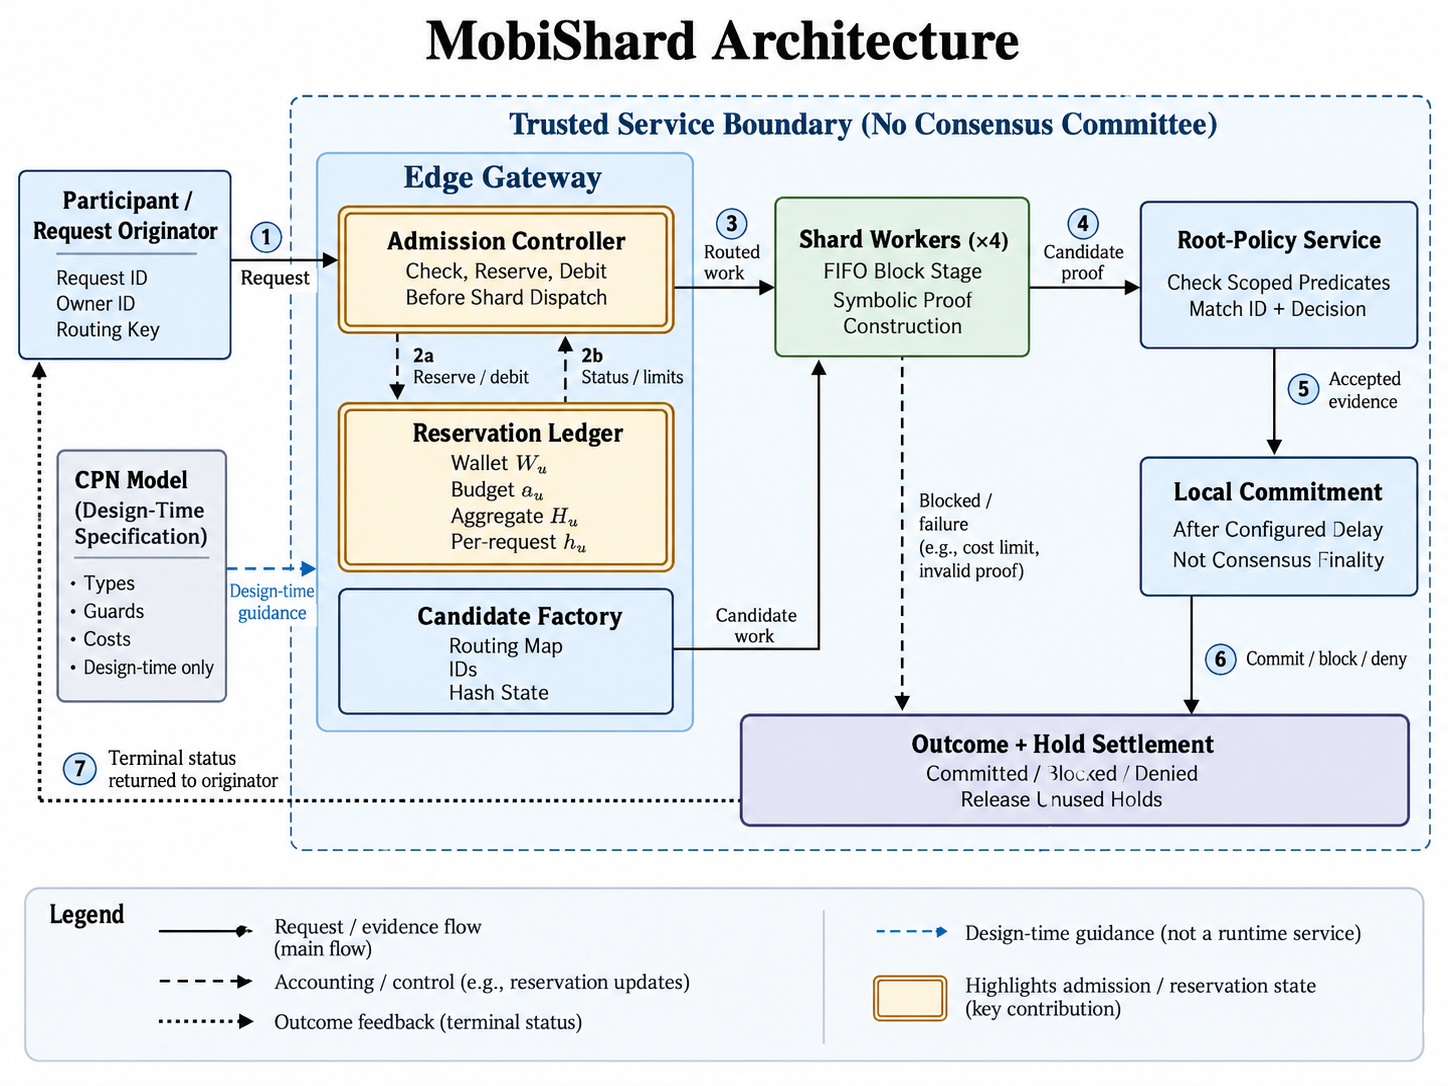
\includegraphics[width=\textwidth]{figures/MobiShard_Architecture.png}
\caption{MobiShard service allocation. The edge gateway maintains admission,
reservation, and candidate-construction state. Four logical shard workers
schedule block-stage calls and construct symbolic proofs; the root-policy
service checks evidence and records local commitment. Terminal handling
returns outcomes and releases unused reservations. The CPN supplies
design-time rules rather than acting as a runtime service.}
\label{fig:architecture}
\end{figure*}

\subsection{Components and End-to-End Flow}

In Fig.~\ref{fig:architecture}, the participant interface supplies the request
identifier and owner binding. The gateway handles admission before execution
services process the request. It requires a mapped routing key and enough
wallet balance for the deposit. Reservation additionally checks connectivity
and the balance left after outstanding holds are excluded. A successful
decision records the hold and debits the deposit atomically. Otherwise the
gateway denies the request without dispatch, deposit debit, or modeled
validation charge.

The account table records each owner's balances and aggregate reservation.
A separate request ledger records ownership, routing assignment, the remaining
hold, the last charged stage, and terminal status. These records distinguish
what remains in the account from what is available to newly arriving work:
part of the balance may already be promised to unfinished requests. The stage
marker tracks charges rather than completed processing. For example, the
block-stage cost is entered before the configured block delay has elapsed.

Edge packaging precedes worker selection through the fixed routing map. A
worker serializes its block-stage processing and calls the gateway for the
stage check and charge. Candidate construction takes place in the gateway,
which also updates the global and shard-specific identifiers and hash-related
state. The worker waits for the block delay, checks the proof inputs, requests
the proof-stage charge, and constructs a symbolic proof. It sends that proof
and the candidate to the root service. Thus, the worker schedules block
processing but does not itself construct the candidate. The four workers
are processing services, not four blockchains with independent consensus.

At the root service, the candidate and proof identifiers must agree and the
retained root-policy predicates must pass. The service then requests the
root-stage charge and records a positive decision for that candidate. A local
commitment can be recorded after the configured delay only with the candidate
and its matching decision. The terminal outcome returns through the gateway
along the request path. The three outcomes distinguish how far processing
reached: \emph{committed} means that the local record was made;
\emph{blocked} means that an admitted request stopped at a handled resource
or evidence check; and \emph{denied} means that the request never entered
processing. Terminal handling releases the remaining hold. Neither earlier
resource charges nor the admission deposit are refunded.

A reserved budget does not exempt a request from later checks. Modeled
connectivity loss can make the owner ineligible at a subsequent guarded
stage and stop work for which resources are still reserved. The check is
stage-specific: after root acceptance, the local commitment timer does not
test connectivity again. Similarly, a release depends on reaching terminal
handling. The implementation does not automatically recover an unused hold
from an unhandled service failure.

\subsection{Why a Precheck Is Not a Reservation}

Take an owner with 14 computation-budget units and enough battery and wallet
allowance to proceed while connectivity remains stable. Each request needs
3 units for block generation, 2 for proof construction, and 2 for root
validation. Before any charge, a full-path precheck can accept three requests
because each is individually affordable at seven units. Now let all three
execute their block stages, spending 9 units, and let two construct proofs,
spending a further 4. The one unit left cannot pay for either root validation
or the third request's proof. This ordering completes no requests, even though
every executed stage passed its guard and the balance stayed non-negative.

Reservation makes a different admission decision: the first two requests
reserve the combined 14-unit cost and the third is denied. The admitted
requests can then complete under A1--A5. This example describes an allowed
ordering, not a measured run or an unavoidable outcome of prechecking.
A schedule that finishes one request before starting the next can also
produce two commitments. Hence the experiment compares reservation with
serialization as well as unreserved checks; both accounting and execution
order can prevent spending on work that never finishes.

The policies differ in what admission does with the available allowance.
\emph{Stagewise checking} checks routing and the wallet first, leaving
resource and connectivity checks to each charged stage. A \emph{full-path
precheck} additionally tests connectivity and the total path cost before
admission, but leaves the balance unreserved. \emph{Lifecycle reservation}
uses the unreserved balance for that decision and retains a per-request hold
throughout processing. \emph{Per-participant serialization} queues an owner's
requests before the full-path precheck. It waits for the current request's
terminal response before admitting the next, without preventing work from
other owners. All four use the same routing, stage costs, and evidence
conditions.

\subsection{Reservation Rule and Accounting Invariant}

The ordered sequence $J=(b,p,r)$ consists of block generation, proof
construction, and root validation. Writing battery before computation, the
configured stage costs and their total are
\begin{equation}
\begin{aligned}
\vq_b&=(2,3),\quad \vq_p=(1,2),\quad \vq_r=(1,2),\\
\vQ&=\vq_b+\vq_p+\vq_r=(4,7).
\end{aligned}
\label{eq:cost}
\end{equation}

For an active request $x$, $J_x$ contains the remaining stages in order,
excluding any that have already been charged. Its remaining reservation is
$\vh_x$. If $\mathcal A_u$ denotes the active requests charged to owner $u$,
then the per-request and aggregate reservations are
\[
\vh_x=\sum_{j\in J_x}\vq_j,\qquad
\vH_u=\sum_{x\in\mathcal A_u}\vh_x.
\]
The sum is zero when no stages remain. Denied and terminal requests retain
no reservation, and vector comparisons throughout are componentwise.

For a new request from a registered owner, assume a unique request identifier
and a positive deposit $d$. The gateway admits it under Reservation when
\begin{equation}
\begin{aligned}
&\operatorname{mapped}(k)\ \land\ W_u\ge d\ \land\ n_u\ne0\\
&\hspace{2em}\land\ \va_u-\vH_u\succeq\vQ.
\end{aligned}
\label{eq:admit}
\end{equation}

The gateway evaluates this condition and records the following changes in
one atomic operation:
\begin{equation}
W_u\leftarrow W_u-d,\quad \vh_x\leftarrow\vQ,\quad
\vH_u\leftarrow\vH_u+\vQ.
\label{eq:hold}
\end{equation}

The request joins $\mathcal A_u$ with its first stage pending. Admission
changes how the allowance is assigned, not how much has been spent:
$\va_u$ is unchanged.

Only an active request's next stage may be charged, after its input and
evidence checks pass. The gateway evaluates the remaining mutable conditions
and applies the charge atomically:
\begin{equation}
n_u\ne0\ \land\ \va_u\succeq\vq_j\ \land\ \vh_x\succeq\vq_j.
\label{eq:stage-budget}
\end{equation}

A successful check permits the following stage charge:
\begin{equation}
\begin{aligned}
\va_u&\leftarrow\va_u-\vq_j,\\
\vh_x&\leftarrow\vh_x-\vq_j,\qquad
\vH_u\leftarrow\vH_u-\vq_j.
\end{aligned}
\label{eq:spend}
\end{equation}

Charging and advancing the expected stage are one operation. The request
spends its existing reservation; it does not repeat the admission test
against the unreserved balance.

For a handled terminal outcome, the gateway releases whatever reservation
remains:
\begin{equation}
\vH_u\leftarrow\vH_u-\vh_x,\qquad \vh_x\leftarrow\mathbf0.
\label{eq:release}
\end{equation}

Settlement also removes the request from $\mathcal A_u$ and records its
terminal status in the same atomic operation. New work can use the released
allowance, but neither $\va_u$ nor $W_u$ increases. A path for which every
stage has been charged already has $\vh_x=\mathbf0$. That value records
exhaustion of the hold, not acceptance of the candidate: matching evidence
and the local timer are still required for commitment. Algorithm~\ref{alg:reservation}
collects the admission, charging, and settlement steps.

\begin{figure}[t]
\centering
\begin{minipage}{.98\columnwidth}
\hrule\smallskip
\refstepcounter{algorithm}
\textbf{Algorithm \thealgorithm.} Lifecycle reservation and settlement
\label{alg:reservation}
\smallskip
\begin{algorithmic}[1]
\STATE \textbf{Input:} new request $x=(r,u,k)$ from registered owner $u$.
\STATE \textbf{Atomically at the gateway:} check Eq.~\eqref{eq:admit};
\STATE \quad if false, return denied; otherwise apply Eq.~\eqref{eq:hold}
\STATE \quad and initialize the active request's stage state.
\STATE Package the admitted request and route it to its worker.
\FOR{each stage $j$ in block, proof, root order}
\STATE Check the stage's input and evidence conditions.
\IF{a required condition fails}
\STATE Settle as blocked using Eq.~\eqref{eq:release}; \textbf{return}.
\ENDIF
\STATE \textbf{Atomically at the gateway:} require active status
\STATE \quad and the expected stage; test Eq.~\eqref{eq:stage-budget}; if true,
\STATE \quad apply Eq.~\eqref{eq:spend} and record the stage charge.
\IF{the stage charge was refused}
\STATE Settle as blocked using Eq.~\eqref{eq:release}; \textbf{return}.
\ENDIF
\STATE Complete stage processing and carry its evidence forward.
\ENDFOR
\STATE Require the candidate's matching positive root decision.
\STATE Wait for the local commitment delay and record commitment.
\STATE Atomically settle using Eq.~\eqref{eq:release}; return committed.
\end{algorithmic}
\smallskip\hrule
\end{minipage}
\end{figure}

\begin{proposition}[Accounted resource feasibility]
Assume A1--A3, non-negative initial budgets, and initially empty reservations.
If the state changes only through the guarded operations above, every update
preserves
\begin{equation}
\va_u\succeq\vH_u\succeq\mathbf0.
\label{eq:invariant}
\end{equation}
The reservation of each active request also equals the cost of its uncharged
stage suffix. Thus, work on another admitted request cannot consume the
allowance assigned to those remaining configured stages.
\end{proposition}

\begin{proof}
The initial state has no active reservations, so $\vH_u=\mathbf0$.
For admission, the test on unreserved balance permits $\vH_u$ to increase
by $\vQ$ and initializes $\vh_x$ to the full path cost. A stage charge
subtracts the same non-negative vector from $\va_u$, $\vh_x$, and $\vH_u$.
The difference between account balance and aggregate hold is therefore
preserved. Fixed costs and the next-stage check maintain the suffix relation,
and the check on the request's hold prevents a negative reservation.
Settlement subtracts the remaining hold without reducing the account balance.
These operations preserve the aggregate invariant and the per-request
relation by induction. Immediately before the next stage $j$, they give
$\va_u\succeq\vH_u\succeq\vh_x\succeq\vq_j$.
The stage's accounted resources are consequently available regardless of
other correctly charged requests. Evidence validity and continued service
or network availability are separate requirements.
\end{proof}

Let $N_u$ count distinct, mapped requests offered by owner $u$, with
\emph{initial} balances $W_u^0$, $B_u^0$, and $C_u^0$. Each completion
consumes one deposit and the full cost in Eq.~\eqref{eq:cost}. The static
resource-capacity bound is
\begin{equation}
K_u=\min\!\left\{N_u,
\left\lfloor\frac{W_u^0}{d}\right\rfloor,
\left\lfloor\frac{B_u^0}{4}\right\rfloor,
\left\lfloor\frac{C_u^0}{7}\right\rfloor\right\}.
\label{eq:bound}
\end{equation}

An owner that is offline for the whole trial contributes $K_u=0$.
Summing yields $K=\sum_u K_u$ because owners cannot pool their budgets.
Reservation and full-path serialization can reach $K$ when owners remain
continuously online or offline, admitted requests have valid evidence, and
processing is allowed to drain. A failure after a deposit debit or an early
stage charge can instead leave fewer resources for completed work. This
bound concerns how many complete paths the budgets can fund; it says nothing
about throughput or latency and does not guarantee liveness.

Resource costs and delays are configured separately. The edge, block, and
local-commitment delays are 2, 5, and 10 abstract units. Assigning 1\,ms
to a unit gives 17\,ms of configured delay, to which queueing, communication,
predicate execution, and runtime overhead must be added. Section~IV measures
these effects. They cannot be inferred from the resource-capacity bound.

\subsection{CPN Traceability and Evidence Boundary}

The stored CPN has eight pages, 72 places, 21 transitions, and 141 arcs.
These inventory counts include receipt structures that the evaluated path
does not use; they are not reachable-state counts. A hash-pinned model file
provides the cost constants, policy parameters, and 64-entry routing map.
The service code implements selected guards and updates using those inputs
without calling the CPN simulator. Table~\ref{tab:traceability} distinguishes
the specification elements from choices made for their runtime implementation.

\begin{table}[t]
\caption{Traceability of the evaluated path. Runtime reservation and terminal
settlement are implementation mechanisms, not features claimed for the
unchanged CPN specification.}
\label{tab:traceability}
\centering
\footnotesize
\setlength{\tabcolsep}{3pt}
\renewcommand{\arraystretch}{1.10}

\begin{tabularx}{\columnwidth}{@{}
  >{\raggedright\arraybackslash}p{0.29\columnwidth}
  >{\raggedright\arraybackslash}X@{}}
\toprule
Specification anchor &
Retained condition and runtime interpretation\\
\midrule

Request creation and deposit &
Wallet sufficiency and deposit $d=15$; runtime requests have separate unique
identifiers.\\
\addlinespace[2pt]

\texttt{P\_CID2SID} &
Keys 0--63 map to four workers. Reusing a routing key does not reuse a
request identifier.\\
\addlinespace[2pt]

\texttt{P\_MobileRes} and resource guards &
Costs $(2,3)$, $(1,2)$, $(1,2)$ and non-offline stage guards are retained;
full-path reservations are added in the gateway.\\
\addlinespace[2pt]

Candidate and proof stages &
Selected evidence rules are transcribed. Candidate construction in the
gateway and worker scheduling are service-allocation choices.\\
\addlinespace[2pt]

\texttt{VerifiedBC}, \texttt{END} &
Commitment requires a candidate and a matching positive decision.
A failed CPN guard does not produce a negative decision token;
blocked termination is a runtime policy.\\
\addlinespace[2pt]

Commitment and timing &
The configured delay becomes a local timer. Committee consensus and
receipt-finality processing are outside the evaluated path.\\

\bottomrule
\end{tabularx}
\end{table}

The failure path illustrates why this distinction matters. In the CPN, a
false guard disables a binding. The runtime instead treats a handled failed
check as a blocked terminal outcome and releases the unused hold. This
fail-fast rule and the chosen worker schedule retain selected conditions
from the model, not all of its possible executions. Replay can check the
accounting and ordering in recorded traces; it does not establish behavioral
equivalence with the CPN or explore its complete reachable state space.

The evidence boundary is visible in the root predicates. They inspect the
auxiliary deposit record at the head of the proof's transaction list,
checking amount, destination, the sender/owner relation, transaction identity,
and a deterministic proof-binding expression. A target parameter and a
block-identifier threshold are checked as well. The evaluated threshold is
zero, not a measured confirmation depth. The checks cover only the specified
fields; they do not authenticate the full routed payload. Nor do their
string-level signature dependencies perform public-key verification.
Acceptance in this experiment means that those predicates succeeded.
Authenticated requests, replay protection, concrete cryptographic checks,
and a specified consensus/commit protocol would be needed for blockchain
integration. The following evaluation therefore concerns accounted completion
capacity and relative runtime under the four admission policies.

\section{Results and Discussion}
\label{sec:results}

Section~\ref{sec:architecture} gives the conditions under which an admitted
request retains its remaining allowance. The experiments ask whether the
implementation attains the associated completion bound and whether retaining
concurrency is useful compared with per-participant serialization. We vary
concurrency and arrival patterns to examine their effect on completion and
runtime, then change modeled connectivity to test the limit of the accounting
guarantee. As before, a measured commitment is a local record, not blockchain
consensus finality.

\subsection{Deployment and Experimental Design}

The services ran under Python 3.13.5 on a Linux x86\_64 host. The container
exposed five logical processors with a four-CPU-equivalent quota and a 4\,GiB
memory limit. A driver used loopback TCP/JSON to communicate with six separate
service processes: the gateway, four shard workers, and the root service.
Topology, routing, stage costs, delays, and event logging were held constant
across policies. With an abstract unit assigned 1\,ms, edge packaging took
a configured 2\,ms, block generation 5\,ms, and local commitment 10\,ms.
These are experimental settings, not a calibration against a wireless network
or operational blockchain. Gateway code performs each account read, check,
and update without an intervening asynchronous suspension.

A trial offered 256 distinct requests, split into 16 requests for each of
16 owners. Requests reused routing keys from the 64-key map, not their unique
identifiers. We reset logical state between trials while keeping the service
processes running. Twenty seeds selected workload order, mixed-profile owner
assignments, and fault targets where applicable. Within each seed, configuration
order was randomized. Matched policy runs have identical recorded input hashes,
but sharing inputs does not make the runtime schedule deterministic. The
retained data exclude four warm-up runs from the main campaign and a separate
44-trial pilot, leaving 880 trials and 225,280 submissions. The artifact
contains their request responses and gateway events, together with environment
information and source hashes.

The policy definitions are those in Section~\ref{sec:architecture}.
\emph{Stagewise} checks the allowance at each charged stage. \emph{Precheck}
also tests the full path cost before dispatch, but records no hold.
\emph{Reservation} maintains the holds in
Eqs.~\eqref{eq:admit}--\eqref{eq:release}. \emph{Serial} acquires a per-owner
lock before applying the full-path precheck and retains it until the gateway
receives the terminal response, including the local commitment delay.
An occupied lock causes later requests from that owner to wait, not to be
denied for being busy. Requests from other owners can proceed concurrently.

The main experiment combines the four profiles in Table~\ref{tab:profiles}
with four policies and 20 repetitions, yielding 320 trials. The default
arrival pattern is a burst, with at most 16 outstanding service calls per
owner at the driver. The computation-limited concurrency study adds caps of
1, 2, 4, and 8 for a further 320 trials; the cap-16 observations come from
the main experiment. Staggered-arrival and full-scan studies each add 80
computation-limited trials, and later disconnection accounts for the final
80 trials. All studies use exact, fixed costs. Only connectivity changes
in the disconnection study, not the cost vector.

\begin{table}[t]
\caption{Initial logical resource profiles. Balances are per owner;
$K$ is the system-wide bound in Eq.~\eqref{eq:bound}. Each owner offers 16 requests.}
\label{tab:profiles}
\centering\footnotesize
\setlength{\tabcolsep}{3pt}
\renewcommand{\arraystretch}{1.10}
\begin{tabularx}{\columnwidth}{@{}
>{\raggedright\arraybackslash}X rrrr
>{\raggedright\arraybackslash}p{1.42cm}@{}}
\toprule
Profile & $W_u^0$ & $B_u^0$ & $C_u^0$ & $K$ & Connectivity\\
\midrule
Deposit-limited & 100 & 100 & 100 & 96 & All online\\
Computation-limited & 300 & 100 & 35 & 80 & All online\\
Battery-budget-limited & 300 & 20 & 100 & 80 & All online\\
Mixed & \multicolumn{3}{c}{Four owner groups} & 96 & One group offline\\
\bottomrule
\end{tabularx}
\par\smallskip\raggedright
Mixed: four owners in each group, with $(W_u^0,B_u^0,C_u^0)$ equal to
$(300,100,100)$, $(300,100,35)$, $(300,20,100)$, or $(300,100,100)$ with
continuous offline status. Their per-owner bounds are 14, 5, 5, and 0,
respectively, giving $K=4(14+5+5)=96$.
\end{table}

\subsection{Metrics and Validation Controls}

Every submission in the retained data has a terminal response: committed,
blocked after admission, or denied before dispatch. Denote these counts by
$N_c$, $N_b$, and $N_d$, respectively, and the number admitted by $N_a$.
They satisfy
\[
N=N_c+N_b+N_d,\qquad N_a=N_c+N_b.
\]
Completion over submissions is $N_c/N$, whereas completion over admissions
is $N_c/N_a$. The latter applies only for $N_a>0$ and excludes denied
requests rather than treating them as successes. For static profiles, we
also compare $N_c$ with $K$. Attaining that resource bound need not make
all 256 offered requests feasible.

Trial elapsed time begins at workload start and ends when all terminal
responses have reached the driver. Request latency begins when the driver
actually releases that request to its concurrency limiter and ends at its
terminal response. It includes waits at the limiter, the gateway's owner
lock, and downstream services, but excludes scheduling delay between a
nominal arrival and actual driver release. For each trial, we calculate
the mean and linearly interpolated 95th percentile of successful-request
latencies, then average those summaries in the timing table. The P95 column
is therefore an average of trial percentiles, not a percentile computed
from pooled requests. Policies may complete different subsets, so these
success-conditioned distributions do not measure latency effects on matched
individual requests.

We measure partial-work cost as the computation allowance charged to requests
that subsequently become blocked:
\[
U_C=\sum_{x:\,\mathrm{outcome}(x)=\mathrm{blocked}} C_x^{\mathrm{spent}}.
\]
Charges are recorded before the associated stage delays finish. Accordingly,
$U_C$ counts configured accounting units, not CPU time or physical energy.
No modeled validation cost is charged to denied requests, although processing
their denials takes time within the trial.

In operational mode, each policy uses constant-work local account checks.
Aggregate reservations are fully reconstructed only after the timed interval
and by a separate replay checker. The diagnostic study moves a full
request-ledger scan into the execution path after every successful admission,
stage charge, and terminal settlement, for all policies. Both modes keep
logging and local assertions enabled. Their timings thus remain measurements
of an instrumented prototype rather than an uninstrumented production
system.

Nineteen unit tests passed. Read-only replay by a separate checker covered
781,126 gateway events from all 880 trials. Checks included balances,
admission eligibility, stage order, deposit debits, unused-reservation
settlement, and non-overlap of an owner's requests under serialization.
For the 77,929 recorded commitments, replay also checked matching positive
decisions and the configured commitment delay. None of these checked
properties was violated in the retained traces. This provides evidence
about those implementation executions, not exhaustive CPN reachability
or model--code equivalence.

The tables give trial means and, where indicated, sample standard deviations.
Selected policy comparisons pair trials by workload seed and use 95\%
Student-$t$ intervals,
$\bar\Delta\pm t_{0.975,19}s_\Delta/\sqrt{20}$.
Analysis is at the trial level; its 256 correlated requests are not independent
replications. These individual intervals are unadjusted and assume independent
trial differences with an adequate $t$ approximation. They characterize
repeatability on this host, rather than performance across deployments or
statistical equivalence of the policies.

\begin{table*}[t]
\caption{Main operational-mode outcomes per 256-request trial, over 20 repetitions.
Committed counts are mean $\pm$ sample standard deviation; other entries are means.
$U_C$ is computation-budget units charged to blocked requests.}
\label{tab:outcomes}
\centering\small
\begin{tabular}{llrrrrr}
\toprule
Profile & Policy & Admitted & Committed & Blocked & Denied & $U_C$\\
\midrule
\tableinput results/paper/outcome_rows.tex
\bottomrule
\end{tabular}
\end{table*}

\subsection{Completion Capacity and Partial-Work Loss}

The deposit-limited profile checks a case in which reservation should add
no completions. Each owner can pay six deposits, giving
$K=16\lfloor100/15\rfloor=96$. All policies admit and complete 96 requests
and deny 160 (Table~\ref{tab:outcomes}). The wallet check has already limited
the work before battery or computation budgets can constrain validation.

For computation-limited owners, the bound is $K=16\lfloor35/7\rfloor=80$.
Stagewise and Precheck fall short, with mean completions of 72.40 and 72.35,
respectively; Reservation and Serial complete 80 in every repetition.
The paired Reservation-minus-Stagewise difference is 7.60 requests, with a
95\% interval of $[6.83,8.37]$, corresponding to a 10.5\% increase over
the Stagewise mean. The burst explains the weak result for Precheck:
all 256 requests in Stagewise or Precheck pass admission before the first
block-stage charge. Nothing has yet been spent or reserved when their
balances are checked. Reservation instead admits 80 and denies 176 before
validation. Serial reaches the same counts by waiting for each owner's
current request to terminate before checking the next.

Figure~\ref{fig:outcomes} also shows what the completion counts exclude.
Reservation completes 100\% of admitted requests, but only
$80/256=31.25\%$ of submissions; the corresponding Stagewise figure is
28.28\%. The submission-level gain is 2.97 percentage points, not 100\%
completion of the offered workload. To explain the shortfall, Stagewise
charges a mean of 46.45 computation units to blocked requests and leaves
6.75 units unused across owners. Its accounting reconciles as
$7(72.40)+46.45+6.75=560$: completed work, partial spending, and residual
balances account for the initial budget. Both the partial charges and the
unusable residual allowance contribute to completing fewer than 80 requests.
Reservation and Serial charge no computation allowance to blocked work.

\begin{figure}[t]
\centering
\begin{tikzpicture}
\begin{axis}[width=\columnwidth,height=5.6cm,ybar stacked,bar width=21pt,
 symbolic x coords={Stagewise,Precheck,Reservation,Serial},xtick=data,
 ymin=0,ymax=275,ytick={0,64,128,192,256},ylabel={Requests per trial},
 tick label style={font=\footnotesize},label style={font=\footnotesize},
 legend style={font=\scriptsize,at={(.5,1.03)},anchor=south,legend columns=3,draw=none},
 axis x line*=bottom,axis y line*=left,enlarge x limits=.16]
\addplot[fill=black!65,draw=black] table[x=policy,y=committed,col sep=comma]{results/paper/cpu_outcomes.csv};
\addplot[pattern=north east lines,draw=black] table[x=policy,y=blocked,col sep=comma]{results/paper/cpu_outcomes.csv};
\addplot[fill=white,draw=black] table[x=policy,y=denied,col sep=comma]{results/paper/cpu_outcomes.csv};
\legend{Committed,Blocked,Denied}
\end{axis}
\end{tikzpicture}

\caption{Computation-limited mean outcomes. Each stacked bar accounts for 256
submissions; its committed and blocked portions together form the admitted
count. Reservation and Serial both reach the 80-request resource bound.}
\label{fig:outcomes}
\end{figure}

The same effect appears when the logical battery budget is binding.
Stagewise completes 72.45 requests on average; Reservation and Serial
complete 80. The change of binding component is an accounting experiment,
not a measurement of device energy. In the mixed profile, Reservation and
Serial reach 96, while Stagewise completes 90.75 and Precheck 90.25.
Precheck denies the 64 requests from initially offline owners, but it still
allows online owners' requests to make overlapping claims on an unreserved
balance. In each profile, the configuration determines the bound and the
measurements show whether the admission policy reaches it.

\subsection{Concurrency, Arrival Patterns, and Serialization}

We next vary the number of outstanding driver calls per owner to examine
the effect of overlap. The cap counts calls waiting for the Serial lock as
well as calls being processed; it is not a bound on successful admissions.
At cap 1, every policy completes 80 requests (Fig.~\ref{fig:concurrency}).
Stagewise still admits requests after usable allowance is exhausted, but
these fail before the block-stage charge, giving $U_C=0$. At caps 2, 4, 8,
and 16, its mean completions decline to 77.15, 75.00, 73.15, and 72.40.
Precheck follows the same general trend. Reservation and Serial remain at
80, although the increased driver cap does not change Serial's one-active-
request restriction for each owner.

\begin{figure}[t]
\centering
\begin{tikzpicture}
\begin{axis}[width=\columnwidth,height=5.8cm,xmode=log,log basis x=2,
 xtick={1,2,4,8,16},xticklabels={1,2,4,8,16},xmin=.85,xmax=18,ymin=70,ymax=81,
 xlabel={Maximum in-flight requests per owner},ylabel={Committed requests per trial},
 tick label style={font=\footnotesize},label style={font=\footnotesize},
 legend style={font=\scriptsize,at={(.98,.02)},anchor=south east,draw=none},
 axis x line*=bottom,axis y line*=left]
\addplot[black,mark=square*,error bars/.cd,y dir=both,y explicit] table[x=cap,y=mean,y error=ci,col sep=comma]{results/paper/concurrency_stagewise.csv};
\addplot[black,dashed,mark=triangle*,error bars/.cd,y dir=both,y explicit] table[x=cap,y=mean,y error=ci,col sep=comma]{results/paper/concurrency_precheck.csv};
\addplot[black,thick,mark=o,mark size=3pt] table[x=cap,y=mean,col sep=comma]{results/paper/concurrency_reserve.csv};
\addplot[black,densely dotted,mark=+,mark size=2pt] table[x=cap,y=mean,col sep=comma]{results/paper/concurrency_serial.csv};
\legend{Stagewise,Precheck,Reservation,Serial}
\end{axis}
\end{tikzpicture}

\caption{Computation-limited mean completions against the per-owner driver cap.
Error bars are 95\% trial-mean intervals. Cap-16 observations are reused from the
main experiment. Reservation and Serial coincide at 80; equal counts do not
imply equal elapsed time.}
\label{fig:concurrency}
\end{figure}

Spacing nominal arrivals 2\,ms apart across the same 256-request stream
raises mean completions to 75.70 for Stagewise and 77.10 for Precheck.
Reservation and Serial still complete 80. More admission checks now occur
after earlier spending becomes visible, which helps Precheck without making
it equivalent to a reservation. The nominal span from the first arrival to
the last is 510\,ms and is included in trial elapsed time. Burst and
staggered trial durations therefore reflect different offered-load patterns.

The capacity result must be read separately from timing. At cap 16 in the
computation-limited profile, Reservation takes a mean of 207.8\,ms per trial
and Serial 205.8\,ms. The paired Reservation-minus-Serial difference is
2.0\,ms, with a 95\% interval of $[-8.0,12.1]$\,ms. This interval does
not establish a timing advantage or show equivalence. In this configuration,
serialization reaches the bound without a demonstrated runtime penalty for
forbidding overlap within an owner.

Mixed resources provide a clearer timing distinction at the same completion
count. Both policies complete 96 requests, but mean trial times are
220.6\,ms for Reservation and 377.2\,ms for Serial. The paired
Serial-minus-Reservation difference is 156.6\,ms, with a 95\% interval of
$[144.9,168.3]$\,ms. An owner in the least constrained group can afford
14 requests. Under Reservation, these paths can overlap; under Serial,
the next request waits until the terminal response releases the owner lock.
This is consistent with the shorter trial time, although the measurements
do not isolate individual scheduling components. The result describes how
long the complete workload, including denials, takes to drain. It does not
imply that every individual request has lower latency.

\subsection{Runtime Instrumentation and Connectivity Loss}

Table~\ref{tab:timing} separates operational accounting from the diagnostic
cost of scanning the request ledger during execution. Full scans increase
mean computation-limited trial time from 234.4 to 260.0\,ms for Stagewise
and from 235.8 to 255.4\,ms for Precheck. For Reservation, the means are
207.8 and 207.4\,ms, giving a paired full-minus-operational difference of
$-0.4$\,ms with a 95\% interval of $[-14.0,13.1]$\,ms. That estimate
cannot be taken as a speedup from extra checking. Scans add work to account
updates and may alter the schedule; the aggregate timing does not separate
these effects. We therefore compare policies using the common local-check
mode and report full-scan timings as a separate diagnostic study. The other
supplementary study changes connectivity after admission.

\begin{table}[t]
\caption{Computation-limited timing in ms. Trial elapsed times are mean $\pm$
sample standard deviation. Latency columns average per-trial successful-request
means and 95th percentiles in operational mode.}
\label{tab:timing}
\centering\footnotesize
\setlength{\tabcolsep}{3pt}
\begin{tabular}{lrrrr}
\toprule
Policy & Operational & Full scan & Mean lat. & P95 lat.\\
\midrule
\tableinput results/paper/timing_rows.tex
\bottomrule
\end{tabular}
\end{table}

The later-disconnection trial begins with every owner online and with wallet,
battery, and computation balances of 300, 100, and 100 units. The workload
seed selects four owners. For each selected owner, the runtime sets its
connectivity flag to offline when its first successfully charged block stage
finishes the configured delay, before that request attempts a proof-stage
charge. The services and loopback connections keep running, so they can
return blocked responses and release unused reservations. The fault changes
the connectivity condition in A5, not the transport connection, and does
not test recovery from a service crash. Root commitment retains its configured
timer and does not recheck connectivity after acceptance.

Table~\ref{tab:disconnect} reports Reservation's 224 admissions, 168
commitments, 56 blocked requests, and 32 denials. Serial completes 168
from 172 admissions, with four blocked requests and 84 denials.
Unaffected owners each support 14 requests, giving $12\times14=168$
commitments; affected owners stop before completion. Serial exposes one
admitted request per affected owner, then denies subsequent requests at
the connectivity precheck. Reservation has already admitted 14 per
affected owner, leaving more unfinished work exposed to the change.

\begin{table}[t]
\caption{Later-disconnection mean outcomes per 256-request trial over 20
repetitions. $U_C$ is computation-budget units charged to blocked requests.}
\label{tab:disconnect}
\centering\footnotesize
\setlength{\tabcolsep}{3.3pt}
\begin{tabular}{lrrrrr}
\toprule
Policy & Admitted & Committed & Blocked & Denied & $U_C$\\
\midrule
\tableinput results/paper/disconnect_rows.tex
\bottomrule
\end{tabular}
\end{table}

Only 75\% of Reservation's admissions complete after the fault, although both
policies complete $168/256=65.625\%$ of submissions. Blocked counts are not
proportional to consumed allowance: $U_C$ is 14.70 for Reservation and 12.00
for Serial, despite 56 versus four blocked requests. Many encounter the
offline condition before any resource charge. Terminal handling releases
unused holds, not spent resources or deposit debits. The invariant remains
satisfied, but more admitted paths can no longer proceed.

\subsection{Interpretation, Limitations, and Deployment Implications}

These results distinguish admission limits from losses during execution.
When the wallet pays for too few deposits, all policies stop admitting work
before validation resources become scarce. When the validation allowance
binds instead, concurrent requests can pass every stagewise check yet leave
spending on paths that do not finish. Reservation avoids that overcommitment;
per-participant serialization reaches the same capacity by waiting between
requests. The remaining choice is whether the time saved by permitting
overlap warrants the larger set of in-flight obligations. The mixed-profile
timing result shows a benefit, and the connectivity experiment shows the
associated exposure.

The workloads contain synthetic deposit and identity records, use fixed
routing, and assign the same stage-specific costs to every request. Costs
differ by stage, not by request or trial. The experiments do not cover
contract-state conflicts, variable bytecode paths, heterogeneous transaction
costs, or estimation error. Overestimating a cost could deny otherwise
feasible work; underestimating it would invalidate the fixed-cost feasibility
argument. In addition, all duties charge a single logical owner. Handling
separately owned device, shard, and root budgets would require a multi-account
mechanism and its own evaluation.

Centralized accounting and candidate-state management may make the gateway
a bottleneck. Atomic event-loop updates do not provide replication or crash
tolerance. The reservation mechanism has neither leases nor recovery, and
settlement depends on reaching handled termination. A protocol that released
an apparently abandoned hold would also have to prevent delayed work from
spending the allowance after release. Changing the modeled offline flag
does not test that situation. Similarly, the valid symbolic records used
in the performance workloads establish neither payload authenticity nor
Byzantine agreement or cross-shard atomicity.

The single-host deployment excludes wide-area communication, mobile radio
behavior, measured energy, and independent-host scaling. Logical resets
and randomized configuration order cannot rule out host-state carryover
from reused processes. Timing remains instrumented and workload-dependent;
intervals over 20 repetitions do not establish production performance.
Replay checks observed accounting and ordering, not all possible executions.
The evidence supports completion-bound attainment under the successful-path
assumptions and useful concurrency in some workloads. It establishes
neither production blockchain throughput nor completion of every admitted
request.


\section{Conclusion}
\label{sec:conclusion}

A non-negative balance is not enough to protect completion under concurrent
validation. Requests may spend their available allowance on early stages and
leave too little for the rest of the path. MobiShard records the remaining
cost as a reservation before shard dispatch, keeping the charged account
separate from the execution host. Under fixed costs and the specified atomic
updates, the invariant prevents one admitted request from using another's
reserved allowance. That accounting protection operates alongside, rather
than in place of, evidence and connectivity checks.

Across 880 trials comparing four policies, Reservation and per-participant
serialization both reached the configured capacity bound in the tested static
profiles without resource-related partial-work loss. In computation-limited
bursts, they each completed 80 of 256 submissions, compared with a Stagewise
mean of 72.40. Equal completion counts leave concurrency, not additional
capacity, as the reason to choose reservation. It reduced mean trial elapsed
time in the mixed profile, while the main computation-limited comparison
showed no clear timing advantage. It also exposed more admitted requests
to interruption when modeled connectivity changed. The evaluation thus
identifies both a use for overlapping validation and a cost to accepting
more work in advance.

The findings concern logical budgets and local commitment in a trusted,
single-host prototype. Further work will address variable cost estimates,
separately owned budgets, and reservation leases with recovery rules that
prevent delayed work from spending released allowance. Concrete cryptographic
verification and consensus are needed before blockchain-level guarantees
can be evaluated. Reservation preserves budget for concurrent validation;
completion still depends on valid evidence, connectivity at guarded stages,
and responsive services.

\bibliographystyle{IEEEtran}
\bibliography{references}
\end{document}
